\section{
    Diferencie os escalonamentos preemptivos e não-preemptivos.
}

\setlength{\parindent}{4em}
\setlength{\parskip}{0.5em}
\renewcommand{\baselinestretch}{1}

% \begin{figure}[h]
%     \centering
%     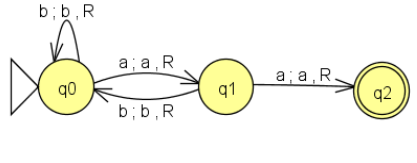
\includegraphics[width=0.65\textwidth]{ex1.png}
%     \caption{Máquina de Turing M.}
%     \label{fig:ex1}
% \end{figure}

Um algoritmo de escalonamento não preemptivo escolhe um processo para executar e vai deixá-lo executando até que ele termine, bloqueie ou que voluntariamente libere a CPU, ou seja, ele não vai suspender o processo em execução.

Um algoritmo preemptivo pode suspender o processo em execução. Ele tem algum tipo de controle de uso da CPU, seja por tempo, por ciclo de clock ou qualquer outro tipo de controle. Ao acabar seu tempo de uso, ele bloqueia o processo e escolhe um outro processo para usar a CPU.